\subsection{Minh chứng thực thi qua giao diện FeatureJ}
\label{sec:gui_evidence}
Bên cạnh lần xuất 72 bản đồ bằng API, một phiên GUI riêng đã được thực hiện
trên ImageJ 1.54p dùng các JAR cài trong Fiji và plugin FeatureJ build từ nguồn
chính thức. Phiên này mở các lớp plugin thật, điền điều khiển trong hộp thoại
và kích hoạt sự kiện OK bằng AWT. Vì vậy, đây là thao tác GUI được tự động hóa,
không phải các bước bấm chuột thủ công và cũng không phải hình minh họa dựng lại.
Ảnh được chụp từ cửa sổ của chính tiến trình Java bằng PrintWindow.

Mỗi phép thử đọc lại PNG gốc, chuyển sang 32-bit, đặt kích thước pixel bằng 1
và đơn vị pixel. Không dùng kết quả phép lọc trước làm đầu vào phép lọc sau.
Các tham số tỷ lệ được lấy từ config của repo. Bảng~\ref{tab:gui_parameters}
ghi cấu hình quan sát được trong các hộp thoại thật.

\begin{table*}[t]
\centering
\caption{Bốn phép thử GUI bổ sung; số đầu ra là số TIFF 32-bit đã lưu.}
\label{tab:gui_parameters}
\begin{tabular}{llp{8cm}r}
\toprule
Lệnh & Ảnh & Tham số & Đầu ra\\
\midrule
Derivatives & bsds\_01 & $x=1$, $y=z=0$, smoothing $=2$ & 1\\
Hessian & drive\_01 & smoothing $=2$; largest và smallest bật; absolute comparison tắt & 2\\
Laplacian & blob\_01 & smoothing $=2$; compute bật; zero-crossings tắt & 1\\
Structure & bsds\_01 & smoothing $=1$, integration $=3$; largest và smallest bật & 2\\
\bottomrule
\end{tabular}
\end{table*}

\begin{figure*}[t]
\centering
\begin{minipage}{0.47\textwidth}
\centering
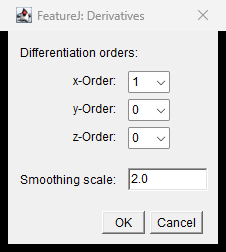
\includegraphics[height=4.6cm]{figures/gui/gui_01_derivatives_dialog.png}
\par (a) Derivatives: $L_x$, $\sigma=2$.
\end{minipage}
\hfill
\begin{minipage}{0.47\textwidth}
\centering
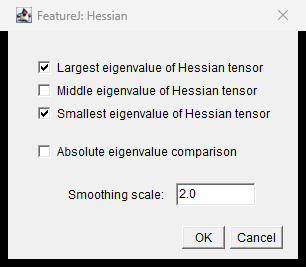
\includegraphics[height=4.6cm]{figures/gui/gui_02_hessian_dialog.png}
\par (b) Hessian: giữ dấu trị riêng.
\end{minipage}
\par\medskip
\begin{minipage}{0.47\textwidth}
\centering
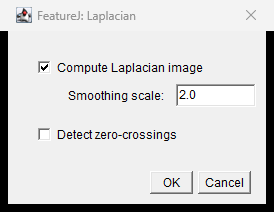
\includegraphics[height=4.3cm]{figures/gui/gui_03_laplacian_dialog.png}
\par (c) Laplacian: không lấy zero-crossings.
\end{minipage}
\hfill
\begin{minipage}{0.47\textwidth}
\centering
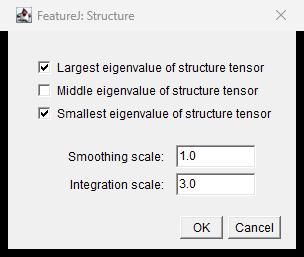
\includegraphics[height=4.3cm]{figures/gui/gui_04_structure_dialog.png}
\par (d) Structure: hai tỷ lệ khác nhau.
\end{minipage}
\caption{Bốn hộp thoại FeatureJ thật trong phiên GUI bổ sung. Các lựa chọn
được đặt trước khi kích hoạt OK; không sử dụng ảnh vẽ lại giao diện.}
\label{fig:gui_dialogs}
\end{figure*}

\begin{figure}[htbp]
\centering
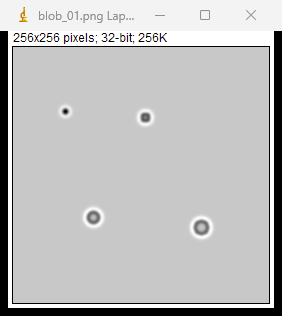
\includegraphics[width=0.72\columnwidth]{figures/gui/gui_03_laplacian_result.png}
\caption{Kết quả Laplacian thật trên blob\_01 tại $\sigma=2$.
Các đốm và vòng đổi dấu minh họa đáp ứng bậc hai; ảnh này chưa phải
kết quả phát hiện blob đa tỷ lệ hoặc kết quả ghép với Ground Truth.}
\label{fig:gui_laplacian}
\end{figure}

Nhật ký \texttt{gui\_capture\_log.csv} ghi bốn lệnh, tham số, thời điểm UTC,
số đầu ra và phương thức chụp. Tổng cộng có sáu TIFF 32-bit trong
\texttt{Code/experiments/gui\_evidence}. Chúng tách khỏi
\texttt{sample\_local}, nơi lưu 72 cặp dùng để chấm sai số.
Phiên GUI xác nhận plugin nhận đúng cấu hình và tạo kết quả;
nó không bổ sung một benchmark F1 mới và không thay thế bộ đối chiếu API.
Đầu ra Derivatives và Laplacian ở đây chưa nhân hệ số chuẩn hóa theo tỷ lệ;
khi đối chiếu với bản đồ đã chuẩn hóa phải áp dụng cùng quy ước
$\sigma^n$ cho đạo hàm bậc $n$.


Đối chiếu TIFF GUI với API trên toàn ảnh cho $L_x$ sai số cực đại bằng 0;
Laplacian so với tổng $L_{xx}+L_{yy}$ có sai số cực đại
$1.90735\times10^{-6}$ và RMSE $4.18613\times10^{-8}$.
Đây là kiểm tra hai phép thử cùng thư viện, không phải so sánh độc lập với NumPy.
